
\documentclass[t]{beamer}
\usetheme{Copenhagen}
\setbeamertemplate{headline}{} % remove toc from headers
\beamertemplatenavigationsymbolsempty

\usepackage{amsmath, tikz, pgfplots, tcolorbox, array, bm, xcolor, colortbl}
\usetikzlibrary{calc}
\pgfplotsset{compat = 1.16}

\tikzstyle{input} = [circle, text centered, radius = 1cm, draw = black]
\tikzstyle{function} = [rectangle, text centered, minimum width = 2cm, minimum height = 1cm, draw = black]

\title{Inverse Functions}
\author{}
\date{}

\AtBeginSection[]
{
  \begin{frame}
    \frametitle{Objectives}
    \tableofcontents[currentsection]
  \end{frame}
}

\begin{document}

\begin{frame}{}
    \maketitle
\end{frame}

\section{Find the inverse of a function}

\begin{frame}{Inverse of an Ordered Pair}
The \alert{inverse} of the ordered pair $(x,y)$ is $(y,x)$.
\end{frame}

\begin{frame}{Example 1}
Find the inverse of each.	\newline\\
(a) \quad $(2,-7)$	\quad \pause $(-7,2)$	\newline\\	\pause
(b) \quad $(0,3)$ \quad \pause $(3,0)$
\end{frame}

\begin{frame}{Review of Functions}
Recall that a function is nothing more than a machine that	\newline\\
\begin{enumerate}
	\item Accepts an input, $x$	\newline\\	\pause
	\item Performs some operation(s)	\newline\\	\pause
	\item Gives an output, $y$	\newline\\	\pause
\end{enumerate}
The inverse function is somewhat of an {\color{blue}``undo"} function.	\newline\\	\pause
It allows us to take the output of a function, put it into our inverse function, and get our original input value back.
\end{frame}

\begin{frame}{Visualization}
Suppose we put a value of 10 into the function \[f(x) = x^2\]	\pause
If we put the output (100) into the inverse, we get our 10 back.	\newline\\	\pause
\begin{center}
    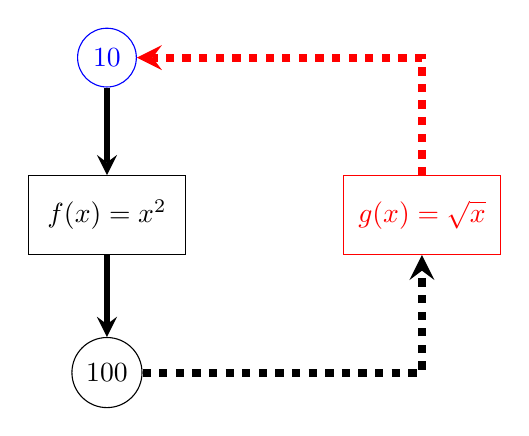
\begin{tikzpicture}[node distance = 2cm]
\node (inputVal) [input, color=blue] {\color{blue}10};
\node (func) [function, below of = inputVal] {$f(x)=x^2$};
\node (outputVal) [input, below of = func] {100};
\node (invFunc) [function, right of = func, xshift = 2cm, color=red] {\color{red}$g(x)=\sqrt{x}$};

\draw [->, >=stealth, thick, line width = 0.75mm] (inputVal) -- (func);
\draw [->, >=stealth, thick, line width = 0.75mm] (func) -- (outputVal);
\draw [->, >=stealth, thick, dashed, line width = 1mm] (outputVal) -| (invFunc);
\draw [->, >=stealth, thick, dashed, line width = 1mm, color = red] (invFunc) |- (inputVal);
\end{tikzpicture}
\end{center}
\end{frame}

\begin{frame}{Inverse Notation}
We use the notation \[f^{-1}(x)\] to denote the inverse of $f(x)$.	\newline\\	\pause

\alert{Note:} The notation {\color{blue}\textbf{does not mean}} raise the function to the $-1$ power.
\end{frame}

\begin{frame}{Steps in Finding the Inverse of a Function}
\begin{enumerate}
	\item Rewrite $f(x)=$ as $y=$	\newline\\	\pause
	\item Switch your $x$ and $y$ variables.	\newline\\	\pause
	\item Solve this result for $y$ and rewrite using inverse notation.
\end{enumerate}
\end{frame}

\begin{frame}{Example 2}
Find the inverse of each of the following.	\newline\\
(a)	\quad	$f(x) = 5x$
\begin{align*}
\onslide<2->{y &= 5x} \\[6pt]
\onslide<3->{x &= 5\alert{y}} \\[6pt]
\onslide<4->{\frac{x}{5} &= \alert{y}} \\[8pt]
\onslide<5->{f^{-1}(x) &= \frac{x}{5}}
\end{align*}
\end{frame}

\begin{frame}{Example 2}
(b) \quad $f(x) = 3x+2$
\begin{align*}
\onslide<2->{y &= 3x+2} \\[6pt]
\onslide<3->{x &= 3\alert{y} + 2} \\[6pt]
\onslide<4->{x-2 &= 3\alert{y}} \\[6pt]
\onslide<5->{\frac{x-2}{3} &= \alert{y}} \\[8pt]
\onslide<6->{f^{-1}(x) &= \frac{x-2}{3}}
\end{align*}
\end{frame}

\begin{frame}{Example 2}
(c) \quad $f(x) = \dfrac{x+5}{7}$
\begin{align*}
\onslide<2->{y &= \frac{x+5}{7}} \\[8pt]
\onslide<3->{x &= \frac{\alert{y}+5}{7}} \\[8pt]
\onslide<4->{7x &= \alert{y} + 5} \\[6pt]
\onslide<5->{7x-5 &= \alert{y}} \\[6pt]
\onslide<6->{f^{-1}(x) &= 7x-5}
\end{align*}
\end{frame}

\begin{frame}{Example 2}
(d)	\quad	$g(x) = x^3 + 1$
\begin{align*}
\onslide<2->{y &= x^3 + 1} \\[8pt]
\onslide<3->{x &= \alert{y}^3 + 1} \\[8pt]
\onslide<4->{x-1 &= \alert{y}^3} \\[8pt]
\onslide<5->{\sqrt[3]{x-1} &= \alert{y}} \\[8pt]
\onslide<6->{g^{-1}(x) &= \sqrt[3]{x-1}}
\end{align*}
\end{frame}

\begin{frame}{Example 2}
(e) 	\quad	$h(x) = 4x^5 - 1$
\begin{align*}
\onslide<2->{y &= 4x^5 - 1} \\[8pt]
\onslide<3->{x &= 4\alert{y}^5 - 1} \\[8pt]
\onslide<4->{x+1 &= 4\alert{y}^5} \\[8pt]
\onslide<5->{\frac{x+1}{4} &= \alert{y}^5} \\[8pt]
\onslide<6->{\sqrt[5]{ \frac{x+1}{4} } &= \alert{y}} \\[8pt]
\onslide<7->{h^{-1}(x) &= \sqrt[5]{\frac{x+1}{4}}}
\end{align*}
\end{frame}

\begin{frame}{Example 2}
(f)		\quad	$f(x) = \sqrt{x+3}$
\begin{align*}
\onslide<2->{y &= \sqrt{x+3}} \\[6pt]
\onslide<3->{x &= \sqrt{\alert{y}+3}} \\[6pt]
\onslide<4->{x^2 &= \alert{y}+3} \\[6pt]
\onslide<5->{x^2-3 &= \alert{y}} \\[6pt]
\onslide<6->{f^{-1}(x) &= x^2 - 3}
\end{align*}
\end{frame}

\begin{frame}{Example 2}
(g)	\quad	$g(x) = \dfrac{5}{x}$
\begin{align*}
\onslide<2->{y &= \frac{5}{x}} \\[8pt]
\onslide<3->{x &= \frac{5}{\alert{y}}} \\[8pt]
\onslide<4->{x\alert{y} &= 5} \\[8pt]
\onslide<5->{\alert{y} &= \frac{5}{x}} \\[8pt]
\onslide<6->{g^{-1}(x) &= \frac{5}{x}}
\end{align*}
\end{frame}

\begin{frame}{Visual Interpretation of Inverse Functions}
Visually, when finding the inverse of a function, you are {\color{blue}\textbf{reflecting that function across the line $\bm{y = x}$}}.	
\end{frame}

\begin{frame}{Visual Interpretation of Inverse Functions}
Below are the graphs of $f(x) = 3x^3-1$ and $f^{-1}(x) = \sqrt[3]{\frac{x+1}{3}}$ as well as the line $y=x$:	\newline\\
\begin{center}
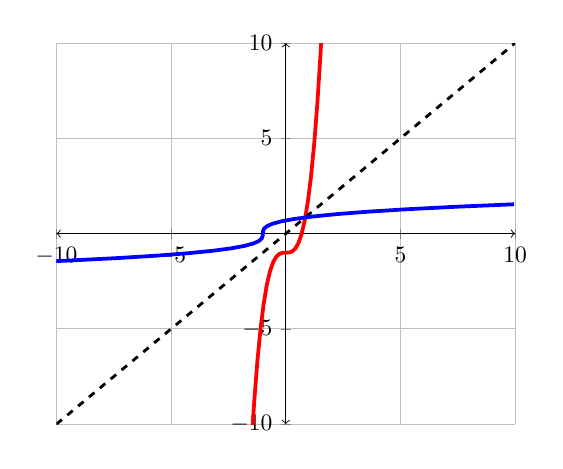
\begin{tikzpicture}[scale=0.85]
\begin{axis}[
	axis lines = middle,
	 axis line style=<->,
	grid,
	xmin = -10, xmax = 10,
	ymin = -10, ymax = 10
	]
	\addplot[color=red, ultra thick, domain=-1.65:1.65] {3*x^3-1};
	\addplot[color=black, very thick, dashed, domain=-10:10] {x};
	\addplot[color=blue, ultra thick, domain=-1.54:1.54] ({3*x^3-1},{x});
\end{axis}
\end{tikzpicture}
\end{center}
\end{frame}

\section{State the Domain and Range of an Inverse Function}

\begin{frame}{Domain and Range of Inverse Functions}
When switching the $x$ and $y$ in finding the inverse function, you also switch the domain and range of the function and its inverse.		\newline\\	\pause

When you graph a function and its inverse, {\color{blue}\textbf{you'll want to make sure that they are reflections across the line $y=x$}}. This is VERY IMPORTANT for a function such as $y = x^2$.	\newline\\	\pause

This might mean we need to \alert{restrict the domain and/or range} of our original function.
\end{frame}

\begin{frame}[c]{Relationship Between Domain and Range}
\[\text{Domain of }f = \text{Range of }f^{-1}\]
\[\text{and}\]
\[\text{Range of }f = \text{Domain of }f^{-1}\]
\end{frame}

\begin{frame}{Example 3}
Find the domain and range of both the function and its inverse.	\newline\\
(a) \quad $f(x) = 5x$	\quad	\onslide<2->{$f^{-1}(x)=\frac{x}{5}$} \newline\\
\begin{center}
\setlength{\extrarowheight}{6pt}
\begin{tabular}{c|c|c}
	&	\textbf{Domain ($\bm{x}$)}	&	\textbf{Range ($\bm{y}$)} \\ \hline
$f(x)$ 			& \onslide<3->{\cellcolor{yellow!75} $\bm{\mathbb{R}}$}	& \onslide<6->{\cellcolor{green!60} $\bm{\mathbb{R}}$}	\\[6pt] \hline
$f^{-1}(x)$	& \onslide<5->{\cellcolor{green!60} $\bm{\mathbb{R}}$}		& \onslide<4->{\cellcolor{yellow!75} $\bm{\mathbb{R}}$}
\end{tabular}
\end{center}
\end{frame}

\begin{frame}{Example 3}(b) \quad $f(x) = 3x+2$	\quad	\onslide<2->{$f^{-1}(x)=\frac{x-2}{3}$} \newline\\
\begin{center}
\setlength{\extrarowheight}{6pt}
\begin{tabular}{c|c|c}
	&	\textbf{Domain ($\bm{x}$)}	&	\textbf{Range ($\bm{y}$)} \\ \hline
$f(x)$ 			& \onslide<3->{\cellcolor{yellow!75} $\bm{\mathbb{R}}$}	& \onslide<6->{\cellcolor{green!60} $\bm{\mathbb{R}}$}	\\[6pt] \hline
$f^{-1}(x)$	& \onslide<5->{\cellcolor{green!60} $\bm{\mathbb{R}}$}		& \onslide<4->{\cellcolor{yellow!75} $\bm{\mathbb{R}}$}
\end{tabular}
\end{center}
\end{frame}

\begin{frame}{Example 3}
(c)	\quad $g(x) = \sqrt{x+3}$ \quad \onslide<2->{$g^{-1}(x) = x^2 - 3$}	\newline\\
\begin{center}
\setlength{\extrarowheight}{6pt}
\begin{tabular}{c|c|c}
					&	\textbf{Domain ($\bm{x}$)}											&	\textbf{Range ($\bm{y}$)} \\ \hline
$g(x)$ 			& \onslide<3->{\cellcolor{yellow!75} $\bm{x \geq -3}$}	& \onslide<5->{\cellcolor{green!60} $\bm{y \geq 0}$}	\\[6pt] \hline
$g^{-1}(x)$	& \onslide<6->{\cellcolor{green!60} $\bm{x \geq 0}$}	& \onslide<4->{\cellcolor{yellow!75} $\bm{y \geq -3}$}
\end{tabular}
\end{center}
\end{frame}

\begin{frame}{Example 3}
(d) \quad $f(x) = -\sqrt{x-4}+2$
\begin{align*}
\onslide<2->{y &= -\sqrt{x-4}+2} \\[6pt]
\onslide<3->{x &= -\sqrt{\alert{y}-4}+2} \\[6pt]
\onslide<4->{x-2 &= -\sqrt{\alert{y}-4}} \\[6pt]
\onslide<5->{-x+2 &= \sqrt{\alert{y}-4}} \\[6pt]
\onslide<6->{(-x+2)^2 &= \alert{y} - 4} \\[6pt]
\onslide<7->{(-x+2)^2+4 &= \alert{y}} \\[6pt]
\onslide<8->{f^{-1}(x) &= (-x+2)^2+4}
\end{align*}
\end{frame}

\begin{frame}{Example 3d}
$f(x) = -\sqrt{x-4}+2$	\quad $f^{-1}(x) = (-x+2)^2+4$	\newline\\
\begin{center}
\setlength{\extrarowheight}{6pt}
\begin{tabular}{c|c|c}
					&	\textbf{Domain ($\bm{x}$)}											&	\textbf{Range ($\bm{y}$)} \\ \hline
$g(x)$ 			& \onslide<2->{\cellcolor{yellow!75} $\bm{x \geq 4}$}	& \onslide<4->{\cellcolor{green!60} $\bm{y \leq 2}$}	\\[6pt] \hline
$g^{-1}(x)$	& \onslide<5->{\cellcolor{green!60} $\bm{x \leq 2}$}	& \onslide<3->{\cellcolor{yellow!75} $\bm{y \geq 4}$}
\end{tabular}
\end{center}
\end{frame}

\begin{frame}{Example 3}
(e)	\quad	$f(x) = x^2$ with $x \geq 0$
\begin{align*}
\onslide<2->{y &= x^2} \\[8pt]
\onslide<3->{x &= \alert{y}^2} \\[8pt]
\onslide<4->{\pm \sqrt{x} &= \alert{y}} \\[8pt]
\onslide<5->{f^{-1}(x) &= \pm \sqrt{x}} \\[8pt]
\end{align*}
\onslide<6->{\emph{Note:} It can NOT be both $\sqrt{x}$ and $-\sqrt{x}$ because it would fail the {\color{blue}\textbf{vertical line test}}.}
\end{frame}

\begin{frame}{Example 3}
$f(x) = x^2$ with $x \geq 0$ \quad $f^{-1}(x) = \pm \sqrt{x}$		\newline\\
\begin{center}
\setlength{\extrarowheight}{6pt}
\begin{tabular}{c|c|c}
					&	\textbf{Domain ($\bm{x}$)}											&	\textbf{Range ($\bm{y}$)} \\ \hline
$g(x)$ 			& \onslide<2->{\cellcolor{yellow!75} $\bm{x \geq 0}$}	& \onslide<4->{\cellcolor{green!60} $\bm{y \geq 0}$}	\\[6pt] \hline
$g^{-1}(x)$	& \onslide<5->{\cellcolor{green!60} $\bm{x \geq 0}$}	& \onslide<3->{\cellcolor{yellow!75} $\bm{y \geq 0}$}
\end{tabular}
\end{center}

\onslide<6->{\[\bm{f^{-1}(x) = \sqrt{x}}\]}
\end{frame}
\end{document}
